% Options for packages loaded elsewhere
\PassOptionsToPackage{unicode}{hyperref}
\PassOptionsToPackage{hyphens}{url}
%
\documentclass[
  10pt,
  letterpaper,
  DIV=11,
  numbers=noendperiod,
  twoside]{scrartcl}

\usepackage{amsmath,amssymb}
\usepackage{setspace}
\usepackage{iftex}
\ifPDFTeX
  \usepackage[T1]{fontenc}
  \usepackage[utf8]{inputenc}
  \usepackage{textcomp} % provide euro and other symbols
\else % if luatex or xetex
  \usepackage{unicode-math}
  \defaultfontfeatures{Scale=MatchLowercase}
  \defaultfontfeatures[\rmfamily]{Ligatures=TeX,Scale=1}
\fi
\usepackage{lmodern}
\ifPDFTeX\else  
    % xetex/luatex font selection
  \setmainfont[ItalicFont=EB Garamond Italic,BoldFont=EB Garamond
Bold]{EB Garamond Math}
  \setsansfont[]{Europa-Bold}
  \setmathfont[]{Garamond-Math}
\fi
% Use upquote if available, for straight quotes in verbatim environments
\IfFileExists{upquote.sty}{\usepackage{upquote}}{}
\IfFileExists{microtype.sty}{% use microtype if available
  \usepackage[]{microtype}
  \UseMicrotypeSet[protrusion]{basicmath} % disable protrusion for tt fonts
}{}
\usepackage{xcolor}
\usepackage[left=1in, right=1in, top=0.8in, bottom=0.8in,
paperheight=9.5in, paperwidth=6.5in, includemp=TRUE, marginparwidth=0in,
marginparsep=0in]{geometry}
\setlength{\emergencystretch}{3em} % prevent overfull lines
\setcounter{secnumdepth}{3}
% Make \paragraph and \subparagraph free-standing
\ifx\paragraph\undefined\else
  \let\oldparagraph\paragraph
  \renewcommand{\paragraph}[1]{\oldparagraph{#1}\mbox{}}
\fi
\ifx\subparagraph\undefined\else
  \let\oldsubparagraph\subparagraph
  \renewcommand{\subparagraph}[1]{\oldsubparagraph{#1}\mbox{}}
\fi


\providecommand{\tightlist}{%
  \setlength{\itemsep}{0pt}\setlength{\parskip}{0pt}}\usepackage{longtable,booktabs,array}
\usepackage{calc} % for calculating minipage widths
% Correct order of tables after \paragraph or \subparagraph
\usepackage{etoolbox}
\makeatletter
\patchcmd\longtable{\par}{\if@noskipsec\mbox{}\fi\par}{}{}
\makeatother
% Allow footnotes in longtable head/foot
\IfFileExists{footnotehyper.sty}{\usepackage{footnotehyper}}{\usepackage{footnote}}
\makesavenoteenv{longtable}
\usepackage{graphicx}
\makeatletter
\def\maxwidth{\ifdim\Gin@nat@width>\linewidth\linewidth\else\Gin@nat@width\fi}
\def\maxheight{\ifdim\Gin@nat@height>\textheight\textheight\else\Gin@nat@height\fi}
\makeatother
% Scale images if necessary, so that they will not overflow the page
% margins by default, and it is still possible to overwrite the defaults
% using explicit options in \includegraphics[width, height, ...]{}
\setkeys{Gin}{width=\maxwidth,height=\maxheight,keepaspectratio}
% Set default figure placement to htbp
\makeatletter
\def\fps@figure{htbp}
\makeatother
% definitions for citeproc citations
\NewDocumentCommand\citeproctext{}{}
\NewDocumentCommand\citeproc{mm}{%
  \begingroup\def\citeproctext{#2}\cite{#1}\endgroup}
\makeatletter
 % allow citations to break across lines
 \let\@cite@ofmt\@firstofone
 % avoid brackets around text for \cite:
 \def\@biblabel#1{}
 \def\@cite#1#2{{#1\if@tempswa , #2\fi}}
\makeatother
\newlength{\cslhangindent}
\setlength{\cslhangindent}{1.5em}
\newlength{\csllabelwidth}
\setlength{\csllabelwidth}{3em}
\newenvironment{CSLReferences}[2] % #1 hanging-indent, #2 entry-spacing
 {\begin{list}{}{%
  \setlength{\itemindent}{0pt}
  \setlength{\leftmargin}{0pt}
  \setlength{\parsep}{0pt}
  % turn on hanging indent if param 1 is 1
  \ifodd #1
   \setlength{\leftmargin}{\cslhangindent}
   \setlength{\itemindent}{-1\cslhangindent}
  \fi
  % set entry spacing
  \setlength{\itemsep}{#2\baselineskip}}}
 {\end{list}}
\usepackage{calc}
\newcommand{\CSLBlock}[1]{\hfill\break\parbox[t]{\linewidth}{\strut\ignorespaces#1\strut}}
\newcommand{\CSLLeftMargin}[1]{\parbox[t]{\csllabelwidth}{\strut#1\strut}}
\newcommand{\CSLRightInline}[1]{\parbox[t]{\linewidth - \csllabelwidth}{\strut#1\strut}}
\newcommand{\CSLIndent}[1]{\hspace{\cslhangindent}#1}

\setlength\heavyrulewidth{0ex}
\setlength\lightrulewidth{0ex}
\usepackage[automark]{scrlayer-scrpage}
\clearpairofpagestyles
\cehead{
  Brian Weatherson
  }
\cohead{
  Four Problems in Decision Theory
  }
\ohead{\bfseries \pagemark}
\cfoot{}
\makeatletter
\newcommand*\NoIndentAfterEnv[1]{%
  \AfterEndEnvironment{#1}{\par\@afterindentfalse\@afterheading}}
\makeatother
\NoIndentAfterEnv{itemize}
\NoIndentAfterEnv{enumerate}
\NoIndentAfterEnv{description}
\NoIndentAfterEnv{quote}
\NoIndentAfterEnv{equation}
\NoIndentAfterEnv{longtable}
\NoIndentAfterEnv{abstract}
\renewenvironment{abstract}
 {\vspace{-1.25cm}
 \quotation\small\noindent\rule{\linewidth}{.5pt}\par\smallskip
 \noindent }
 {\par\noindent\rule{\linewidth}{.5pt}\endquotation}
\KOMAoption{captions}{tableheading}
\makeatletter
\@ifpackageloaded{caption}{}{\usepackage{caption}}
\AtBeginDocument{%
\ifdefined\contentsname
  \renewcommand*\contentsname{Table of contents}
\else
  \newcommand\contentsname{Table of contents}
\fi
\ifdefined\listfigurename
  \renewcommand*\listfigurename{List of Figures}
\else
  \newcommand\listfigurename{List of Figures}
\fi
\ifdefined\listtablename
  \renewcommand*\listtablename{List of Tables}
\else
  \newcommand\listtablename{List of Tables}
\fi
\ifdefined\figurename
  \renewcommand*\figurename{Figure}
\else
  \newcommand\figurename{Figure}
\fi
\ifdefined\tablename
  \renewcommand*\tablename{Table}
\else
  \newcommand\tablename{Table}
\fi
}
\@ifpackageloaded{float}{}{\usepackage{float}}
\floatstyle{ruled}
\@ifundefined{c@chapter}{\newfloat{codelisting}{h}{lop}}{\newfloat{codelisting}{h}{lop}[chapter]}
\floatname{codelisting}{Listing}
\newcommand*\listoflistings{\listof{codelisting}{List of Listings}}
\makeatother
\makeatletter
\makeatother
\makeatletter
\@ifpackageloaded{caption}{}{\usepackage{caption}}
\@ifpackageloaded{subcaption}{}{\usepackage{subcaption}}
\makeatother
\ifLuaTeX
  \usepackage{selnolig}  % disable illegal ligatures
\fi
\usepackage{bookmark}

\IfFileExists{xurl.sty}{\usepackage{xurl}}{} % add URL line breaks if available
\urlstyle{same} % disable monospaced font for URLs
\hypersetup{
  pdftitle={Four Problems in Decision Theory},
  pdfauthor={Brian Weatherson},
  hidelinks,
  pdfcreator={LaTeX via pandoc}}

\title{Four Problems in Decision Theory}
\author{Brian Weatherson}
\date{2024}

\begin{document}
\maketitle
\begin{abstract}
TBC
\end{abstract}

\setstretch{1.1}
Decision theory has become too disjointed. Problems that should be
discussed together have spawned separate literatures. This paper aims to
put the parts back together.

One principle, what I'll call the Single Choice Principle, tightly
constrains the solutions to four separate kinds of problems in decision
theory. These are: how to model rational risk aversion; how to
incorporate evidential connections between options and states; whether
probabilities, values, or options can be non-linear; and, how to relate
synchronic and dynamic choice. In each case, once we accept the Single
Choice Principle, only a narrow range of views are left as viable. By
seeing the connections between these four questions, we also see how to
answer them.

Ultimately, I'll argue for these conclusions, all of them using little
more than the principle I call Single Choice.

\begin{itemize}
\tightlist
\item
  Risk-sensitive alternatives to orthodox expected utility theory, as
  defended by e.g., Buchak (\citeproc{ref-BuchakRisk}{2013}), are
  mistaken.
\item
  The right decision theory for problems involving Demons (e.g.,
  Newcomb's Problem) is a form of causal ratificationism.\footnote{It's
    a version of what Eells and Harper
    (\citeproc{ref-EellsHarper1991}{1991}) call \emph{basic
    ratificationism}.}
\item
  Even if probabilities are linearly ordered (contra Keynes
  (\citeproc{ref-Keynes1921}{1921})), and values of outcomes are
  linearly ordered (contra Chang (\citeproc{ref-Chang2002}{2002})),
  preferences over options are not linearly ordered. This undermines
  many of the arguments that have been made against Keynes and Chang.
\item
  The two main views about dynamic choice, the \emph{sophisticated}
  (\citeproc{ref-Hammond1976}{Hammond 1976}) and \emph{resolute}
  (\citeproc{ref-McClennen1990}{McClennen 1990}), are both half right.
  In cases where the agent's preferences do not change over the course
  of a decision problem\footnote{Cases where they do change are set
    aside for purposes of this paper; see Pettigrew
    (\citeproc{ref-Pettigrew2019}{2019}) for a good discussion of the
    issues that they bring up.}, a choice is rational only if both
  dynamic and resolute approaches would endorse it.
\end{itemize}

In the next two sections I'll set out the Single Choice Principle. The
following five sections will make good on the promises in these bullet
points. (There are five, not four, because I use one section to argue
against linearity of preferences, and then another to relate this back
to the views defended by Keynes and Chang.) I conclude by noting how the
arguments here support a conclusion defended by William Harper
(\citeproc{ref-Harper1984}{1985}, \citeproc{ref-Harper1986}{1986},
\citeproc{ref-Harper1989}{1989}): decision theory should be more like
game theory.

\section{Introducing the Single Choice Principle}\label{sec-scp-intro}

Think about two ways to play chess.

First, we might sit down somewhere, possibly in a park, facing each
other, with a board and some pieces in front of us. We take turns moving
pieces, and eventually someone wins. Probably you; I'm not very good at
chess.

Second, we sit down at our computers, probably not in a park, and write
code to make our computers play chess against each other. We meet,
exchange code, and run the programs against each other to see who wins.
It's still probably you, but my chances would be a bit better in this
form.

In the first version we are playing the \emph{dynamic} form of chess; in
the second we are playing the \emph{strategic} form. In game-theoretic
language, a strategy for a game like chess is a set of instructions
saying what to do in every possible state of the game.\footnote{Standardly,
  this includes states that are ruled out by the earlier parts of the
  strategy.} An explicit strategy for chess, with a conditional saying
\emph{If in state S, make move M} for every possible state \emph{S},
would be unimaginably large. But code for chess computers can be quite
compact; I have a few versions just on my phone.

This is a philosophy paper, so I'm going to take these mundane examples,
idealise them, and evaluate the idealisations.

The idealisation is that I'm going to not assume it's you and me
playing, but two characters who have no computational limitations. I'll
call one of these Chooser.

The evaluation is that for Chooser, some moves are rational and some are
not. This is true whether Chooser is playing the dynamic or the
strategic form.

To start I won't ask what moves are rational, but instead ask about the
connection between the two games. In particular, are the evaluations for
the two games related in the following way.

\begin{description}
\tightlist
\item[Dynamic-Strategic Equivalance (for chess)]
In chess, move \emph{M} at game state \emph{S} in the dynamic game is
rational iff some strategy which includes \emph{If S, do M} is rational
in the strategic game.
\end{description}

This is not an implausible view, in part because of some special
features of chess. Chess includes no random moves by Nature, no
information that is revealed to some players and not others, and it is
zero-sum. By `zero-sum', I mean that there is no pair of players and
pair of game states such that both players are better off in one of the
states than the other.

Games in general need not have any of these features. \emph{Settlers of
Catan}, for example, has none of them. There are random dice rolls and
card draws; while the dice are public, the cards are private; and there
are mutually beneficial trades between players. Some theories say that
in games with these features, especially the last, Dynamic-Strategic
Equivalence can fail. (The other two features will require us to be
careful in how we state Dynamic-Strategic Equivalence.)

Consider a very simplified version of the Ultimatum game. In this
version, the players have \$3 to distribute. As in the standard version,
Proposer will suggest a split of the money, and Respondant will accept
or reject the split. If they reject it, neither player will get any
money. I'll add two more simplifications. First, only proper splits are
allowed; Proposer can't suggest that one or other party gets all the
money. Second, the dollars cannot be split. So the only proposals are
that Proposer gets \$1 and Respondant gets \$2, or that Proposer gets
\$2 and Respondant gets \$1. Call these Proposals P1 and P2.

In this game, Respondant has four possible strategies. I'll write XY for
responding to P1 with X and P2 with Y. So the strategy RA is the (odd)
strategy of rejecting the offer of \$2 and accepting the offer of \$1.
Using this terminology, this version of Ultimatum is given by
Table~\ref{tbl-ultimatum}. (As usual, I'll write the row players payouts
first. This is a little misleading because we normally put the payoff of
the first mover first. But it will fit better with how I'll use the game
in a few paragraph.)

\begin{longtable}[]{@{}rcc@{}}
\caption{Ultimatum game}\label{tbl-ultimatum}\tabularnewline
\toprule\noalign{}
& P1 & P2 \\
\midrule\noalign{}
\endfirsthead
\toprule\noalign{}
& P1 & P2 \\
\midrule\noalign{}
\endhead
\bottomrule\noalign{}
\endlastfoot
AA & \$1, \$2 & \$2, \$1 \\
AR & \$2, \$1 & \$0, \$0 \\
RA & \$0, \$0 & \$1, \$2 \\
RR & \$0, \$0 & \$0, \$0 \\
\end{longtable}

Assuming both players prefer more money to less, there are three Nash
equilibria of this game: (P2, AA), (P2, RA), and (P1, AR). But there is
only one dynamic equilibrium of the game: (P2, AA). In a one-shot
version of the dynamic game, there is no payoff to ever playing R; it's
always a choice between more money and less. So Respondent must play AA,
and so Proposer is best off playing P2.

Let's bring this back to decision theory. Assume that Respondent is
Chooser, our main subject. Assume also that Proposer is Demon, the
familiar character from Newcomb's Problem. Demon, as I'll understand
him, is arbitrarily good at predicting Chooser's \emph{strategy}, and
Chooser knows this.\footnote{If we wanted realistic cases, we would make
  Demon only somewhat good at predicting strategies. It would still be
  possible to get versions of most of the examples here working, but
  they would be more complicated and harder to follow. Making Demon
  arbitrarily good loses some realism, but gains some simplicity.}

Some decisions theories say that this version of Ultimatum violates
Dynamic-Strategic Equivalence (hereafter, just Equivalence). Causal
decision theorists that say Chooser should pick the optimal equilibrium,
e.g., Harper (\citeproc{ref-Harper1984}{1985}) say that Chooser should
play AR in the strategic game, but AA in the dynamic game. Evidential
decision theoriests, e.g., Ahmed (\citeproc{ref-Ahmed2014}{2014}), say
the same thing.

I'm going to ultimately reject these theories, but not because of what
they say about this case. It is not obvious whether Dynamic-Strategic
Equivalence should hold here. As I just noted, some approaches to game
theory say that it should not.\footnote{I think Equivalence does hold
  here because in the strategic game AA is the only option that is not
  weakly dominated. But I'm not going to argue for weak dominance in
  this paper, or work out just how it relates to Equivalence in the
  general case. Here, as often in this paper, I'm indebted to Stalnaker
  (\citeproc{ref-Stalnaker1999}{1999}).}

There is a narrower class of decision problems where Equivalence does
seem intuitively compelling. A strategy in Table~\ref{tbl-ultimatum} is
a pair of conditionals. The strategy says what to do if Demon plays P1,
and what to do if Demon plays P2. Consider the class of decision
problems where a strategy is a single conditional. A strategy in such a
problem says \emph{If we get to this point, do X}. I call these Single
Choice problems. Here's the first statement of the core premise of this
paper.

\begin{description}
\tightlist
\item[Single Choice Principle (SCP)]
In all Single Choice problems, Dynamic-Strategic Equivalence holds.
\end{description}

The intuition behind SCP is simple. In a dynamic Single Choice game, the
only option is what to do at the point choice is called for. Assume X is
a rational move to make at that point. Now think about whether the
strategy \emph{If I reach that point, do X} is rational. Following
Ramsey (\citeproc{ref-RamseyGeneralProp}{{[}1929{]} 1990}), the way to
answer that question is to imagine reaching the point, then asking
whether it is rational to do X. And we just said that it is. So the
strategy is rational. Conversely, if doing X at that point is not
rational in the dynamic game, the same argument will show that the
strategy \emph{If I reach that point, do X} is not rational.

\section{Clarifying the Single Choice Principle}\label{sec-scp-clarify}

Think back to games involving cards. Imagine our hero, Chooser, is
playing a game in which someone else has just drawn a card. In some
sense, the game state is different if the card is an Ace than if it is a
King. But Chooser's strategy cannot depend on that. Chooser can only
react to what they know. So Chooser's strategy cannot be a list of
things about what to do at every game state, in this sense of game
state, where they have to choose.

The standard way game theorists handle this involves the notion of
\emph{information sets}. Say that the different \emph{nodes} of the game
are individuated finely enough that they encode everything that has
happened to that point which could make a difference to the outcome. So
if the other person drew an Ace, that will move the game to a different
node than if they drew a King. Say that some nodes are in the same
information set if (a) the same person must choose at every node in the
set, and (b) at any node in the set, every other node in the set is
compatible with that chooser's information at the time of
choice.\footnote{There is an implicit assumption here that epistemic
  possibility is an equivalence relation. That's too strong and for some
  purposes should be relaxed. It is, however, a harmless enough
  idealisation for the purposes of this paper.} To continue our card
game, if the other player draws a King rather than an Ace, then Chooser
has to move, those moves will take place at different nodes in the same
information set.

This terminology allows for a more perspicuous formulation of SCP.

\begin{description}
\tightlist
\item[Single Choice Principle]
Any decision problem where all the nodes where Chooser must choose are
in a single information set, Dynamic-Strategic Equivalence holds.
\end{description}

I'll work through some examples where SCP applies, and then note an
example where it does not.

Here is a rather boring game. A card will be drawn, and not shown to
Chooser. If it is neither and Ace nor a King, the game ends, as a draw.
(When a game ends, I always assume this is announced to all players.)
Otherwise, Chooser is asked to guess whether it is an Ace or a King. If
they guess correctly, they win, otherwise, they lose. The game tree for
this game is Figure~\ref{fig-ace-king}.

\begin{figure}

\centering{

\includegraphics{fourprob-late-2024_files/figure-pdf/fig-ace-king-1.png}

}

\caption{\label{fig-ace-king}The Ace-King game.}

\end{figure}%

The dashed lines around the two nodes on the right indicates that they
are in the same information set. There are two nodes where Chooser must
choose, but they are in the same information set, so SCP applies. In
this case, SCP is hardly controversial. Either guess is equally rational
in the tree in Figure~\ref{fig-ace-king}, and either guess is equally
rational in the strategic form of the game shown in
Table~\ref{tbl-ace-king}.

\begin{longtable}[]{@{}rccc@{}}
\caption{Strategic form of Ace-King
game}\label{tbl-ace-king}\tabularnewline
\toprule\noalign{}
& Other & Ace & King \\
\midrule\noalign{}
\endfirsthead
\toprule\noalign{}
& Other & Ace & King \\
\midrule\noalign{}
\endhead
\bottomrule\noalign{}
\endlastfoot
Guess Ace & 0 & 1 & -1 \\
Guess King & 0 & -1 & 1 \\
\end{longtable}

Another kind of game where SCP applies is exemplified by Newcomb's
Problem. The standard vignette that goes with Newcomb's Problem suggests
it is a dynamic choice problem. Demon \emph{predicts} what Chooser will
do, and Chooser \emph{then} selects one box or two. The fact that
Demon's predictions changes the content of an \emph{opaque} box means
that the different moves Demon could make lead to different nodes in the
same information set. All this is shown in Figure~\ref{fig-newcomb}.

\begin{figure}

\centering{

\includegraphics{fourprob-late-2024_files/figure-pdf/fig-newcomb-1.png}

}

\caption{\label{fig-newcomb}Newcomb's Problem.}

\end{figure}%

But while this is the standard vignette, it is not the way Newcomb's
Problem is usually represented. Rather, Newcomb's Problem is usually
represented in a table like Table~\ref{tbl-newcomb}, which is a correct
representation of the strategic form of Figure~\ref{fig-newcomb}.

\begin{longtable}[]{@{}rcc@{}}
\caption{Strategic form of Newcomb's
Problem}\label{tbl-newcomb}\tabularnewline
\toprule\noalign{}
& P1 & P2 \\
\midrule\noalign{}
\endfirsthead
\toprule\noalign{}
& P1 & P2 \\
\midrule\noalign{}
\endhead
\bottomrule\noalign{}
\endlastfoot
Choose 1 & 1000 & 0 \\
Choose 2 & 1001 & 1 \\
\end{longtable}

In tables like Table~\ref{tbl-newcomb}, I'll typically have Demon select
the column, and I'll write PX to mean that the Demon predicted X. So
here, `P1' means Demon predicted Chooser would take 1 box.

There is rather a lot of dispute about Newcomb's Problem. To the best of
my knowledge, no party to that dispute says that the difference between
Figure~\ref{fig-newcomb} and Table~\ref{tbl-newcomb} makes a difference
to that dispute. Everyone moves freely between them. This is evidence
that everyone accepts SCP restricted to Newcomb's Problem. If such a
restricted form of SCP holds, then it probably holds somewhat more
broadly. (At the very least, it should still hold if we change the
payoffs.)

So far I've shown how SCP can apply to cases involving gambles, and to
cases involving Demons. The most important applications will involve
mixing those things. In particular, we'll be interested in cases like
Figure~\ref{fig-main-example}.

Figure~\ref{fig-main-example} is a three stage decision problem. At
stage 3, if we get that far, Chooser will select Up or Down. At stage 1,
Demon will predict what Chooser will do at stage 3, again if we get that
far. At stage 2, if Demon predicts Down, nothing happens and we move to
stage 3. But if Demon predicts Up, a biased coin will be flipped. The
coin has probability 3/4 of landing Heads. If it lands Heads, the game
ends, and Chooser gets 0. If it lands Tails, we move to stage 3. Then
after Chooser makes their choice, the payouts are delivered. Chooser
gets nothing if Demon predicted incorrectly; gets 4 if Demon correctly
predicted Up, and 2 if Demon correctly predicted Down.

\begin{figure}

\centering{

\includegraphics{fourprob-late-2024_files/figure-pdf/fig-main-example-1.png}

}

\caption{\label{fig-main-example}The main example of SCP}

\end{figure}%

There is only 1 chice point for Chooser, so the strategy table for
Figure~\ref{fig-main-example} is very simple. It is shown in
Table~\ref{tbl-main-example}.

\begin{longtable}[]{@{}rcccc@{}}
\caption{Strategy table for
Figure~\ref{fig-main-example}}\label{tbl-main-example}\tabularnewline
\toprule\noalign{}
& H \& PU & H \& PD & T \& PU & T \& PD \\
\midrule\noalign{}
\endfirsthead
\toprule\noalign{}
& H \& PU & H \& PD & T \& PU & T \& PD \\
\midrule\noalign{}
\endhead
\bottomrule\noalign{}
\endlastfoot
Up & 0 & 0 & 4 & 0 \\
Down & 0 & 2 & 0 & 2 \\
\end{longtable}

The SCP says that the rationally acceptable moves in
Figure~\ref{fig-main-example} and Table~\ref{tbl-main-example} are the
same. If this wasn't true, we'd get a very weird result. If some
strategy is rational in Table~\ref{tbl-main-example} but not
Figure~\ref{fig-main-example}, then it would be rational for Chooser to
think \emph{If I have to choose, I'm doing X}, and then, after learning
that they have to choose and nothing else, it would be irrational to do
X. Alternatively, if some move X is rational in
Figure~\ref{fig-main-example} but not in Table~\ref{tbl-main-example},
it would be irrational to think \emph{If I have to choose, I'll do X},
even though, after learning that they had to choose and nothing else, it
would be rational to do X. Either way, this seems to violate some
fundamental rules about how conditionals work.

So, I conclude, the SCP is correct. It follows from simple principles
about conditionals, and it explains why, although everything else about
Newcomb's Problem has been contested, no one has argued that the
difference in representation between Figure~\ref{fig-newcomb} and
Table~\ref{tbl-newcomb} matters.

This conclusion, however, turns out to have fairly dramatic consequences
across much of decision theory.

\section{Problem 1: Risk-Sensitivity}\label{sec-buchak}

Think about what value of \emph{x} would make Chooser indifferent
between these two options, and why that would be the right value:

\begin{enumerate}
\def\labelenumi{\arabic{enumi}.}
\tightlist
\item
  \$1,000,000
\item
  A gamble that returns \$2,000,000 with probability \emph{x}, and \$0
  with probability 1-\emph{x}.
\end{enumerate}

What factors are relevant to solving for \emph{x}? One factor is the
declining marginal utility of money. Money primarily has exchange value,
and if Chooser won \$2,000,000, Chooser would exchange the second
million for things they chose not to exchange the first million for, so
the second million has less value. That's one reason that \emph{x} is
well above ½.

But is it the only reason? The orthodox answer is that it is. Lara
Buchak (\citeproc{ref-BuchakRisk}{2013}) has argued that it is not. We
also need to know how much Chooser values, or more likely disvalues,
risk. That is, we need to know how risk-seeking, or risk-averse, Chooser
is.

The orthodox view is that all we need to know are three numbers. In what
follows, let \emph{b} be Chooser's current wealth in millions, and V the
function from wealth (in millions), to utility. Since V is only
determined up to positive affine transformations, we can stipulate two
of these values for V.

\begin{itemize}
\tightlist
\item
  V(\emph{b}), stipulated to be 0.
\item
  V(\emph{b} + 1), stipulated to be 1.
\item
  V(\emph{b} + 2), which we'll label \emph{c}.
\end{itemize}

On the standard view, the gamble's value is \emph{cx}, so Chooser is
indifferent between it and the money iff \emph{x}~=~1/\emph{c}. On
Buchak's view, rational Chooser has a risk function \emph{f}, that
measures their sensitivity to risk. The function must be monotonic
increasing, with \emph{f}(0)~=~0, and \emph{f}(1)~=~1. If Chooser is
risk-averse, then typically \emph{f}(\emph{x})~\textless~\emph{x}.
Buchak's view reduces to the orthodox view if
\emph{f}(\emph{x})~=~\emph{x}. I'm going to argue that given SCP,
\emph{f}(\emph{x}) does equal \emph{x}. I'm far from the first to argue
for \emph{f}(\emph{x})~=~\emph{x}.\footnote{See Briggs
  (\citeproc{ref-Briggs2015}{2015}) and Thoma
  (\citeproc{ref-Thoma2019}{2019}) for different arguments to the same
  conclusion.} What's novel here is drawing this conclusion from just
SCP.

The core of Buchak's theory is a non-standard way of valuing a gamble.
For simplicity, we'll focus on gambles with finitely many outcomes.
Associate a gamble with a random variable \emph{O}, which takes values
\emph{o}\textsubscript{1}, \ldots, \emph{o\textsubscript{n}}, where
\emph{o\textsubscript{j}}~\textgreater~\emph{o\textsubscript{i}} iff
\emph{j}~\textgreater~\emph{i}. Buchak says that the risk-weighted
expected utility of \emph{O} is given by this formula, where \emph{f} is
the agent's risk-weighting function.

\begin{quote}
REU(\emph{O}) = \emph{o}\textsubscript{1} + \(\sum_{i = 2}^n\)
\emph{f}(Pr(\emph{O} ⩾
\emph{o\textsubscript{i}}))(\emph{o\textsubscript{i}} -
\emph{o}\textsubscript{\emph{i}-1})
\end{quote}

The decision rule then is simple: choose the gamble with the highest
REU. The key notion here is the risk function \emph{f}, which we
introduced earlier. I'm going to show that if
\emph{f}(\emph{x})~=~\emph{x}\textsuperscript{2}, then we get a
violation of SCP. I won't go through the details of how this generalises
to all other values of \emph{f} other than identity\footnote{If \emph{f}
  if the identity function, Buchak's way of valuing gambles just becomes
  orthodox expected utility theory}, but it should be easy enough to see
how to use the recipe here to find a problem for any other value of
\emph{f}.

As is standard, I'll assume that random moves in a game are made by a
player called Nature. Chooser is always assumed to know the moves
available to Nature at a node, and the probability that it will make any
given move having arrived at that node.

In Figure~\ref{fig-buchak} at stage 1 a fair die will be rolled. If it
lands 1 or 2, Nature moves Left; if it lands 3 or 4, Nature moves
Middle; otherwise, Nature moves Right. If Nature moves Left, the game
ends, and Chooser gets 1. Otherwise Chooser is told that Nature did not
move Left, but not whether they moved Middle or Right. If Chooser
selects Down, they get 1. If Chooser selects Up, they get 5 if Nature
moved Middle, and 0 otherwise.

\begin{figure}

\centering{

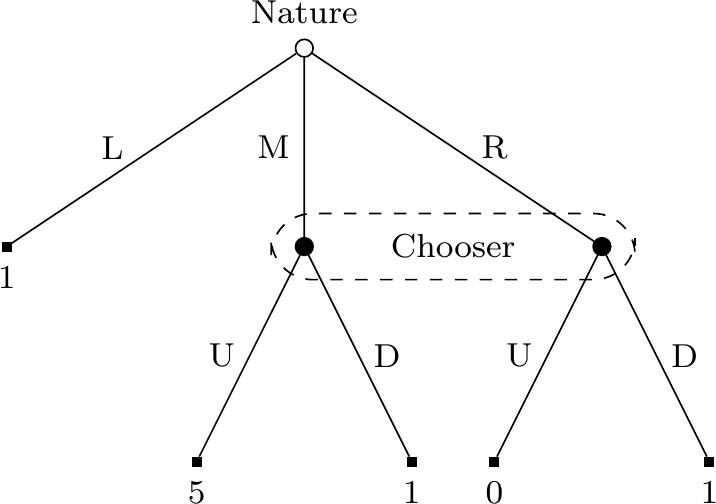
\includegraphics{fourprob-late-2024_files/figure-pdf/fig-buchak-1.png}

}

\caption{\label{fig-buchak}Tree Diagram of the counterexample to REU.}

\end{figure}%

Table~\ref{tbl-buchak-early} shows the strategic table of
Figure~\ref{fig-buchak}, and Table~\ref{tbl-buchak-late} shows the
decision table Chooser faces at the time they have to choose.

\begin{table}

\caption{\label{tbl-panel}Two strategy tables for
Figure~\ref{fig-buchak}.}

\begin{minipage}{0.50\linewidth}

\subcaption{\label{tbl-buchak-early}The strategy table at game start.}

\centering{

\begin{tabular}{cccc}
\toprule
 & \textbf{Left} & \textbf{Middle} & \textbf{Right}\\
\midrule
\textbf{Up} & 1 & 5 & 0\\
\textbf{Down} & 1 & 1 & 1\\
\bottomrule
\end{tabular}

}

\end{minipage}%
%
\begin{minipage}{0.50\linewidth}

\subcaption{\label{tbl-buchak-late}The strategy table at choice time.}

\centering{

\begin{tabular}{ccc}
\toprule
 & \textbf{Middle} & \textbf{Right}\\
\midrule
\textbf{Up} & 5 & 0\\
\textbf{Down} & 1 & 1\\
\bottomrule
\end{tabular}

}

\end{minipage}%

\end{table}%

In Table~\ref{tbl-buchak-early}, the REU of Down is 1 (since that's the
only possible outcome), and the REU of Up is 8/9. There is a 2/3 chance
of getting at least 1, so that's worth 4/9, and there's a 1/3 chance of
getting another 4, so that's also worth 4/9, and adding those gives 8/9.
So the optimal strategy, according to REU theory, is Down. That is, REU
says to prefer the strategy \emph{Choose Down if you have to choose} to
the strategy \emph{Choose Up if you have to choose}. But if we get to
the choice point, we're at Table~\ref{tbl-buchak-late}. And in that
table the REU of Up is 5 times 1/4, i.e., 5/4. So at that point, REU
says to choose Up. What REU says to do if you have to choose is
different to which strategy it chooses for the one and only point you
have to choose at. That is, Buchak's theory violates the SCP, and so
should be rejected.

\phantomsection\label{refs}
\begin{CSLReferences}{1}{0}
\bibitem[\citeproctext]{ref-Ahmed2014}
Ahmed, Arif. 2014. \emph{Evidence, Decision and Causality}. Cambridge:
{C}ambridge {U}niversity {P}ress.

\bibitem[\citeproctext]{ref-Briggs2015}
Briggs, Ray. 2015. {``Costs of Abandoning the Sure-Thing Principle.''}
\emph{Canadian Journal of Philosophy} 45 (5): 827--40. doi:
\href{https://doi.org/10.1080/00455091.2015.1122387}{10.1080/00455091.2015.1122387}.

\bibitem[\citeproctext]{ref-BuchakRisk}
Buchak, Lara. 2013. \emph{Risk and Rationality}. Oxford: Oxford
University Press.

\bibitem[\citeproctext]{ref-Chang2002}
Chang, Ruth. 2002. {``The Possibility of Parity.''} \emph{Ethics} 112
(4): 659--88. doi:
\href{https://doi.org/10.1086/339673}{10.1086/339673}.

\bibitem[\citeproctext]{ref-EellsHarper1991}
Eells, Ellery, and William Harper. 1991. {``Ratifiability, Game Theory,
and the Principle of Independence of Irrelevant Alternatives.''}
\emph{Australasian Journal of Philosophy} 69 (1): 1--19. doi:
\href{https://doi.org/10.1080/00048409112344491}{10.1080/00048409112344491}.

\bibitem[\citeproctext]{ref-Hammond1976}
Hammond, Peter J. 1976. {``Changing Tastes and Coherent Dynamic
Choice.''} \emph{The Review of Economic Studies} 43 (1): 159--73. doi:
\href{https://doi.org/10.2307/2296609}{10.2307/2296609}.

\bibitem[\citeproctext]{ref-Harper1984}
Harper, William. 1985. {``Ratifiability and Causal Decision Theory:
Comments on Eells and Seidenfeld.''} In \emph{PSA 1984}, edited by Peter
Asquith and Philip Kitcher, Two: Symposia and Invited Papers:213--28.
East Lansing, MI: Philosophy of Science Association.

\bibitem[\citeproctext]{ref-Harper1986}
---------. 1986. {``Mixed Strategies and Ratifiability in Causal
Decision Theory.''} \emph{Erkenntnis} 24 (1): 25--36. doi:
\href{https://doi.org/10.1007/BF00183199}{10.1007/BF00183199}.

\bibitem[\citeproctext]{ref-Harper1989}
---------. 1989. {``Decisions, Games and Equilibrium Solutions.''} In
\emph{PSA 1988}, edited by Arthur Fine and Jarrett Leplin, Two: Symposia
and Invited Papers:344--62. East Lansing, MI: Philosophy of Science
Association.

\bibitem[\citeproctext]{ref-Keynes1921}
Keynes, John Maynard. 1921. \emph{Treatise on Probability}. London:
Macmillan.

\bibitem[\citeproctext]{ref-McClennen1990}
McClennen, Edward. 1990. \emph{Rationality and Dynamic Choice}.
Cambridge: {C}ambridge {U}niversity {P}ress.

\bibitem[\citeproctext]{ref-Pettigrew2019}
Pettigrew, Richard. 2019. \emph{Choosing for Changing Selves}. Oxford:
{O}xford {U}niversity {P}ress.

\bibitem[\citeproctext]{ref-RamseyGeneralProp}
Ramsey, Frank. (1929) 1990. {``General Propositions and Causality.''} In
\emph{Philosophical Papers}, edited by D. H. Mellor, 145--63. Cambridge:
Cambridge University Press.

\bibitem[\citeproctext]{ref-Stalnaker1999}
Stalnaker, Robert. 1999. {``Extensive and Strategic Forms: Games and
Models for Games.''} \emph{Research in Economics} 53 (3): 293--319. doi:
\href{https://doi.org/10.1006/reec.1999.0200}{10.1006/reec.1999.0200}.

\bibitem[\citeproctext]{ref-Thoma2019}
Thoma, Johanna. 2019. {``Risk Aversion and the Long Run.''}
\emph{Ethics} 129 (2): 230--53. doi:
\href{https://doi.org/10.1086/699256}{10.1086/699256}.

\end{CSLReferences}



\noindent Published in\emph{
?meta:citation.container-title}, 2024, pp. ?meta:citation.page.

\end{document}
